\section{Results}

\begin{figure}[h!]
  \centering
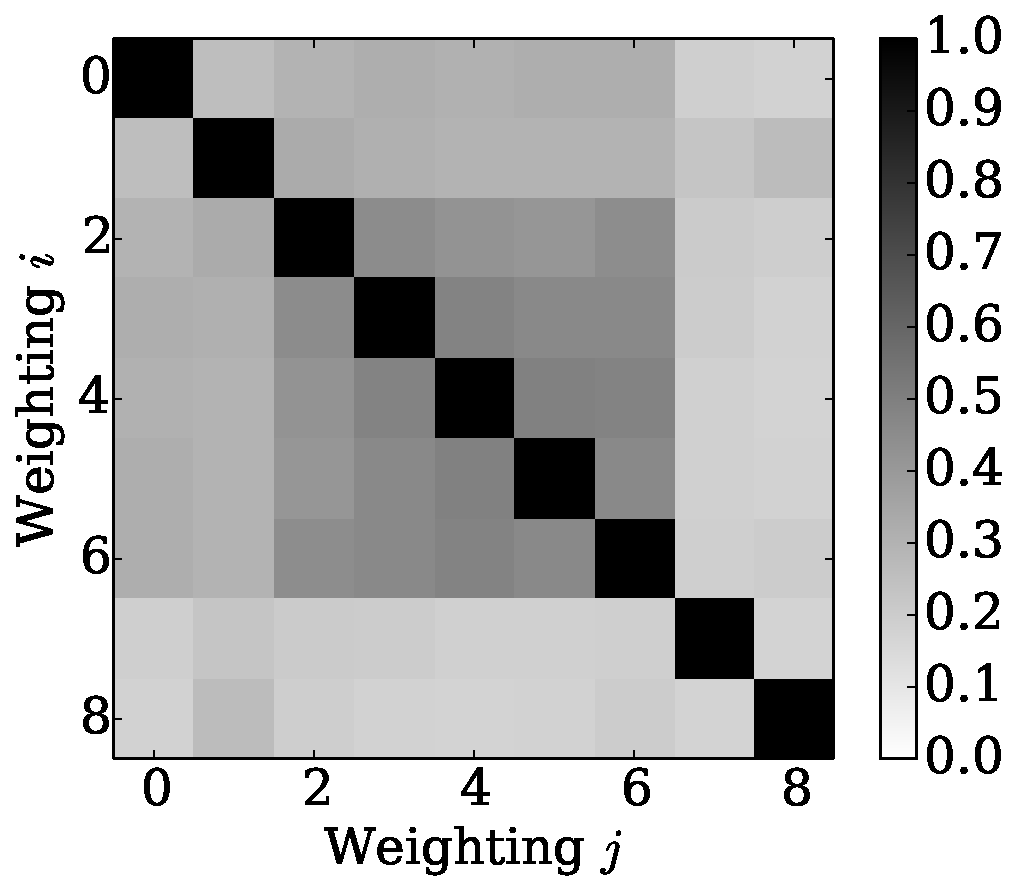
\includegraphics[width=0.50\textwidth]{figures/nmi_no_singletons.pdf}
\caption{The normalized mutual information between the communities using the different weightings. Weighting 0 corresponds to the structural (binary weighting) network, weightings 1 through 6 correspond to the weighting using the transfer entropy with lag 1 through 6, weighting 7 corresponds to the hashtag similarity, and weighting 8 corresponds to the retweet-mention weighting. Values of normalized mutual information close to 1 indicate similarity in the community structure, while values close to 0 indicate dissimilarity. The normalized mutual information is computed with the singletons removed.}
\label{Fig-compare_coverings}
\end{figure}

\begin{figure}[h!]
  \centering
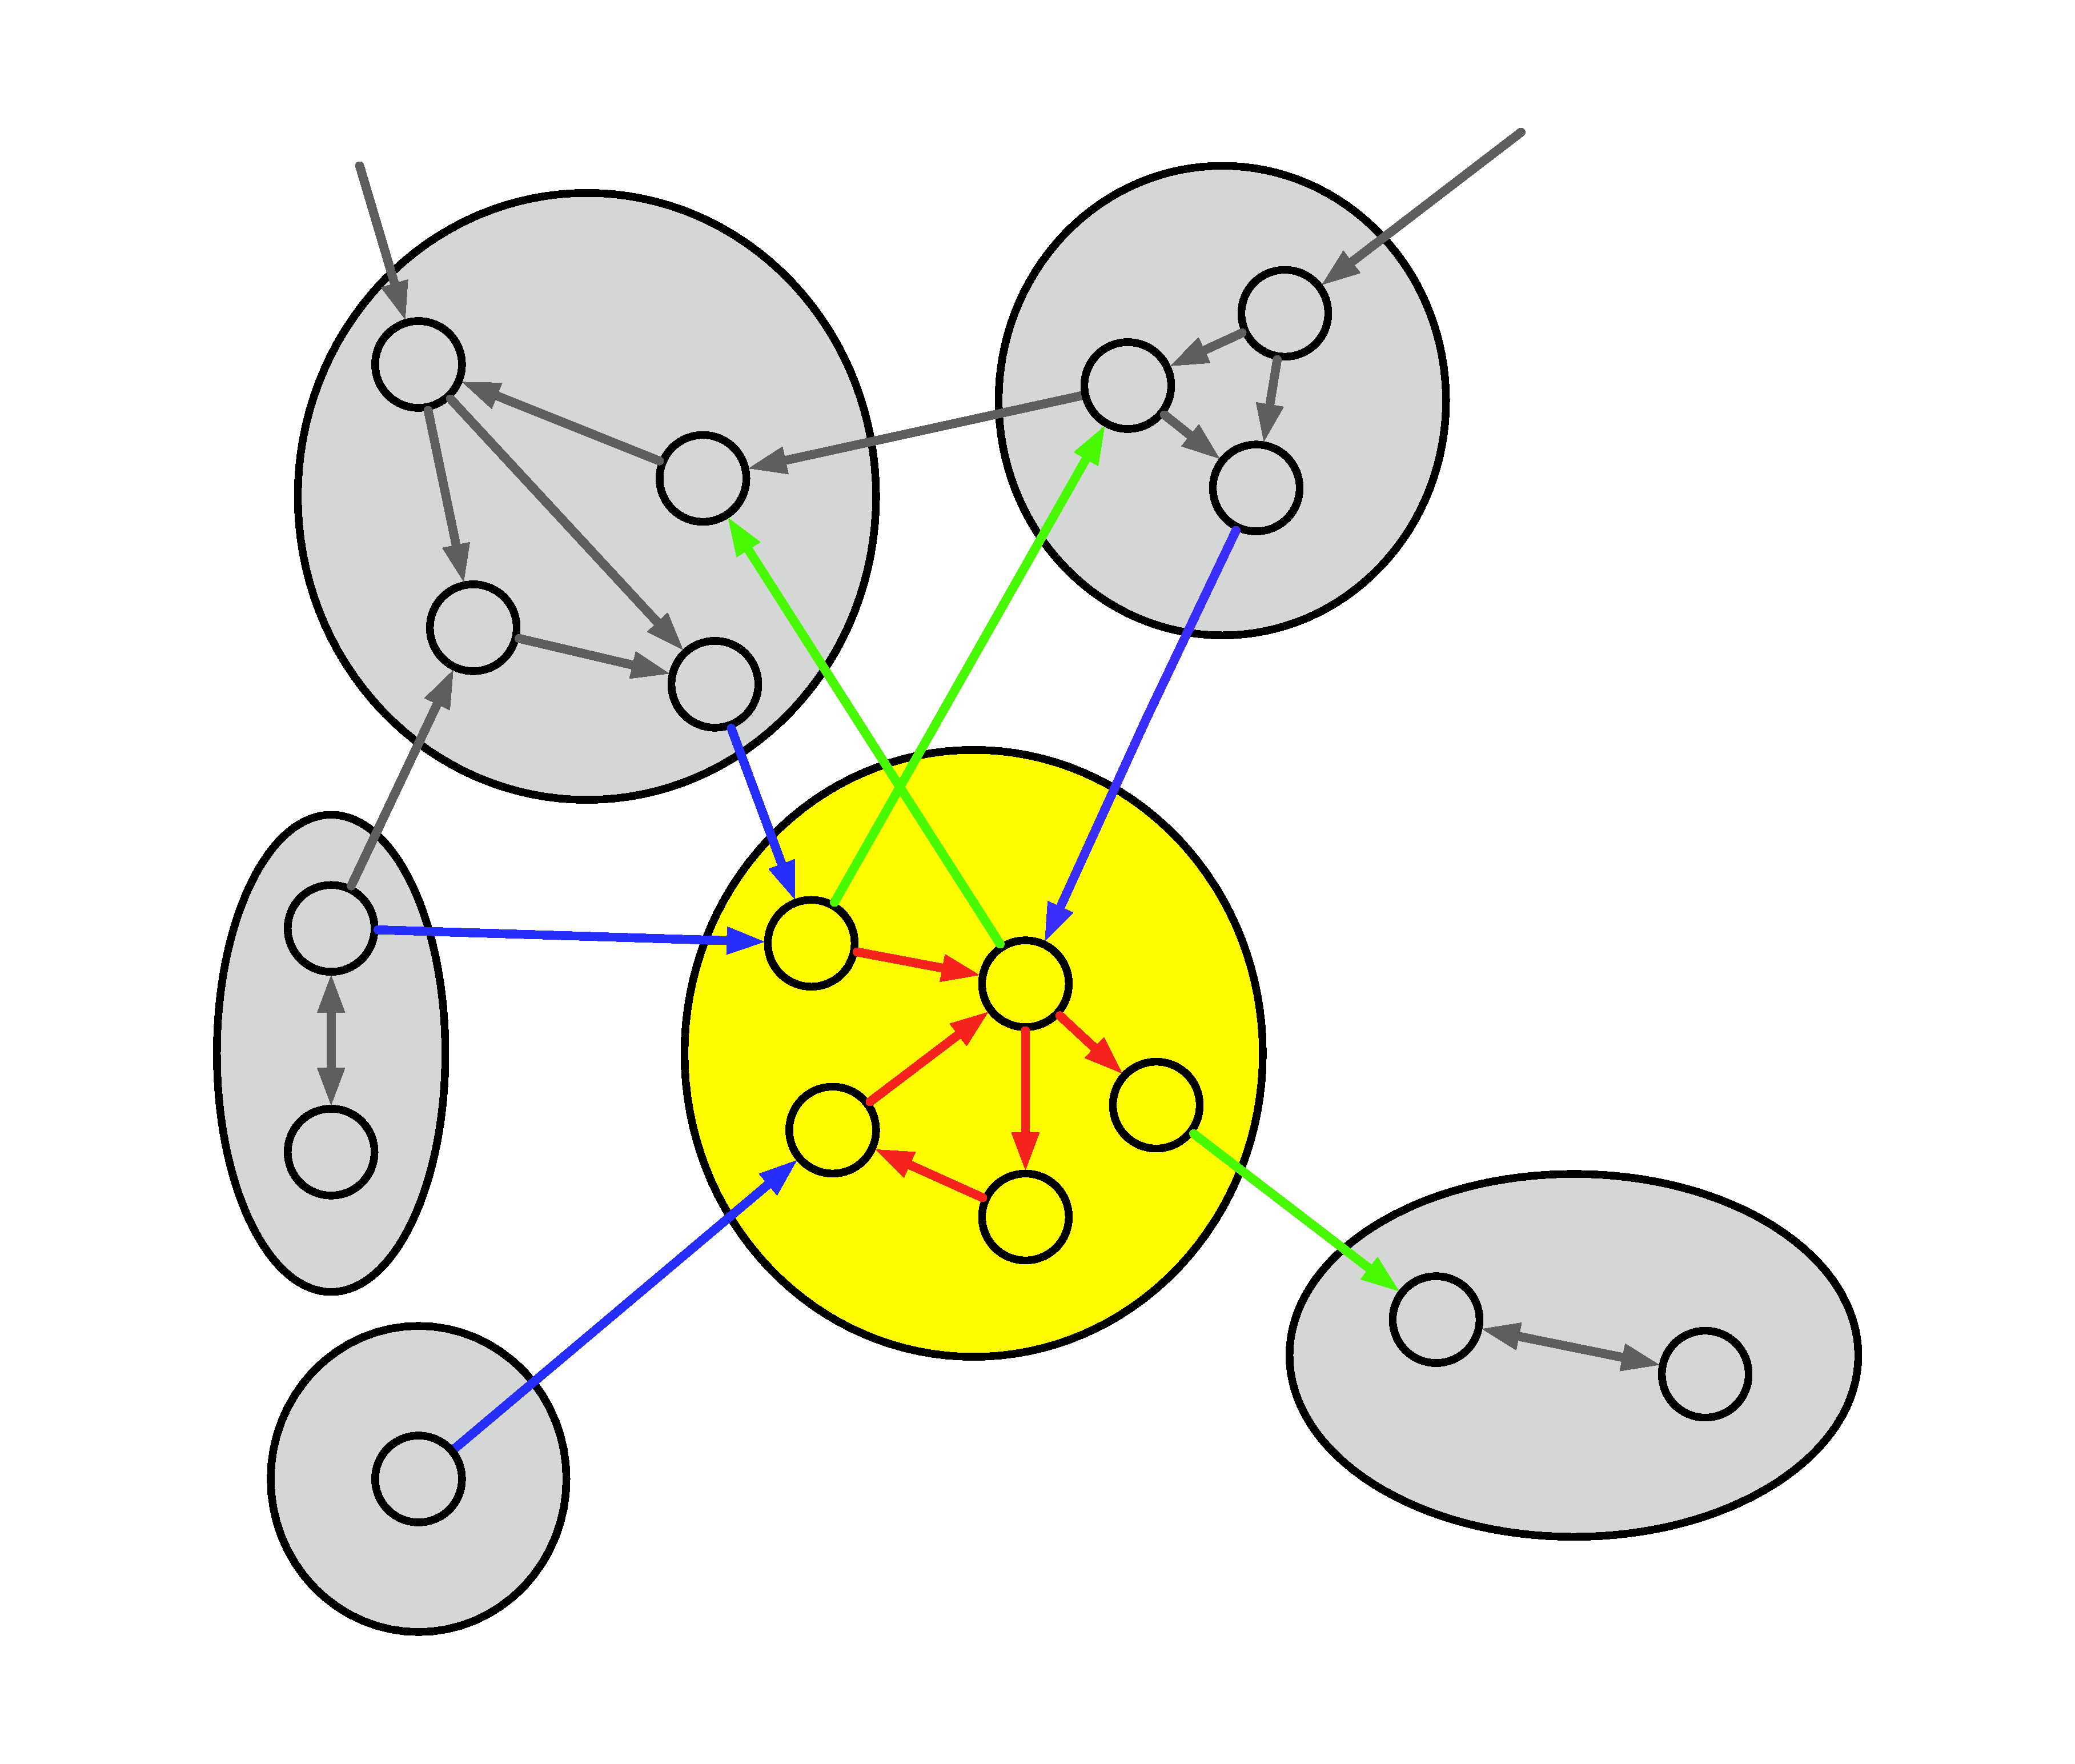
\includegraphics[width=0.50\textwidth]{figures/edge-types.eps}
\caption{An example of the edges considered in determining the edge weight distribution for a given community (the focal community is in yellow). We focus on the internal-to-internal (red), internal-to-external (green), and external-to-internal (blue) edges. For a given focal community, all other edges (grey) are not considered.}
\label{Fig-edge_types}
\end{figure}